\documentclass[11pt]{article}
\usepackage{geometry}
 \geometry{
 a4paper,
 total={170mm,257mm},
 left=20mm,
 top=20mm,
 }
\usepackage{xspace}
\usepackage{tcolorbox}
\tcbuselibrary{listings}
\newtcblisting{code}{
  listing only,
  nobeforeafter,
  after={\xspace},
  hbox,
  tcbox raise base,
  fontupper=\ttfamily,
  colback=lightgray,
  colframe=lightgray,
  size=fbox
  }
\usepackage{tikz}
\usetikzlibrary{shapes.geometric, arrows}
\usetikzlibrary{matrix}
\author{Gerrit Roessler}
\title{Sudoku Solver Technical Specifications}
\date{2023}

\begin{document}
\maketitle
\section{Introduction}
This project takes an input file containing an 
(unsolved) sudoku board in the form of a CSV, and solve it, using Rustlang. This document is made with \LaTeX.
\section{Goals}
\begin{enumerate}
  \item Command line input
  \item Takes input file, generates an output file
  \item Making use of the wave function collapse algorithm.
\end{enumerate}
\subsection{Stretch Goals}
\begin{enumerate}
  \item Graphical User Interface, or GUI
  \item In the case of branching solutions, generating multiple outputs
  \item Threading
  \item GPU Acceleration
\end{enumerate}
\section{Wave Function Collapse}
Wave function collapse is an algorithm that has a scary name, but 
is surprisingly simple, if resource intensive. The idea is that if 
an item has an unknown state (like a sudoku tile that isn't filled in), 
conceptually it can be considered in all of the states it could possibly be in.
For exmpale, given a very simple psudo-sudoku board, only going up to 4 (as opposed to 9):\\
\begin{center}
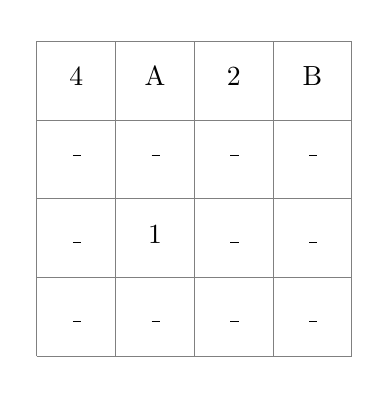
\begin{tikzpicture}
\draw[step=0.5cm,color=gray,xscale=2,yscale=2] (-1,-1) grid (1,1);
\matrix[matrix of nodes,nodes={inner sep=0pt,text width=1cm,align=center,minimum height=1cm}]{
4 & A & 2 & B \\
\_ & \_ & \_ & \_ \\
\_ & 1 & \_ & \_ \\
\_ & \_ & \_ & \_\\};
\end{tikzpicture}
\end{center}
Consider A and B to be tiles that aren't filled in. If only the top row is considered, the wave
function collapse algorithm would say that both $A$ and $B$ are in both a state of being 1 
and a state of being 3, at the same time! But if the program then considers tiles outside the top row,
it sees that in the second column, which $A$ belongs to, there is a 1. Since $A$ now cannot be $\{1, 3\}$, 
instead the set of all its current possible states is $\{3\}$. Because of this, it's real state is known, and it 
"collapses" into a single state, namely being 3. Since $A$ is now 3, the set of all of $B$'s states is now simply
$\{1\}$, meaning it too can collapse into a single state. \\
\section{Large picture process}
\begin{center}
\tikzstyle{startstop} = [rectangle, rounded corners, minimum width=3cm, minimum height=1cm,text centered, draw=black, fill=red!30]
\tikzstyle{io} = [trapezium, trapezium left angle=70, trapezium right angle=110, minimum width=3cm, minimum height=1cm, text centered, draw=black, fill=blue!30]
\tikzstyle{process} = [rectangle, minimum width=3cm, minimum height=1cm, text centered, draw=black, fill=orange!30]
\tikzstyle{decision} = [diamond, minimum width=3cm, minimum height=1cm, text centered, draw=black, fill=green!30]
\tikzstyle{arrow} = [thick,->,>=stealth]

\begin{tikzpicture}[node distance=1.75cm]
  \node (start) [startstop] {Command line perameters};
  \node (pro1) [process, below of=start] {Seek input file};
  \node (dec1) [decision, below of=pro1, yshift=-0.6cm] {Is is usable?};
  \node (stop) [startstop, right of=dec1, xshift=3cm] {Stop, provide error message};
  \node (pro2) [process, below of=dec1, yshift=-0.6cm] {Format input into data structure};
  \node (wfc) [io, below of=pro2] {Wave Function Collapse};
  \node (dec2) [decision, below of=wfc, yshift=-1.5cm] {Is the puzzle solvable?};
  \node (error) [startstop, right of=dec2, xshift=3.6cm] {Stop, provide error message};
  \node (out) [startstop, below of=dec2, yshift=-1.5cm] {Output solved sudoku};

  \draw [arrow] (start) -- (pro1);
  \draw [arrow] (pro1) -- (dec1);
  \draw [arrow] (dec1) -- node[anchor=south] {no} (stop);
  \draw [arrow] (dec1) -- node[anchor=east] {yes} (pro2);
  \draw [arrow] (pro2) -- (wfc);
  \draw [arrow] (wfc) -- (dec2);
  \draw [arrow] (dec2) -- node[anchor=south] {no} (error);
  \draw [arrow] (dec2) -- node[anchor=east] {yes} (out);
\end{tikzpicture}
\end{center}
\section{Why Rust/How Rust?}
The Rust language is ideal for this project for many reasons. Primarily, the type system it offers, combined with the
pattern matching it provides, allows for excellent error handling for avoiding issues at runtime. Secondly, similar to the C family,
Rust is a relatively fast language, which is imperative for this project, due to the nature of the algorithm in use. \\
Because of the Rust compiler and the Rust Foundation's clear stance on what idiomatic Rust looks like, using the common naming conventions shouldn't be an issue.
For example, variables in snake\_case, UpperCamelCase for data structures, SCREAMING\_SNAKE\_CASE for statics, etc. If something isn't idiomatically named, the 
Rust compiler will throw a warning. As with most Rust projects, defining what pardigm is in use is difficult, as Rust provides optionality for everything 
from (something like) OOP to (something like) functional programming. This project will use mainly a OOP design pattern, basing around data 
structures and associated methods, however useful functional features such as closures are encouraged.
Discussing the use of specific crates, command line input is managed by the Clap crate and I/O is managed by the CSV crate. 
If GPU acceleration is achievable within the given timeframe, it seems that the crate WGPU is the most advanced one in rust for GLSL compilation. 
\section{Errors}
Rust does it's very best not to error, and slightly less then it's best not to panic. To achieve this, any time a operation might not complete it's 
operation, it returns the Result enum, in the form of either Ok() or Err(). This is dandy for an aspiring programmer, however different Rust creates (or even sub sections inside
of the standard library) return different, non-uniform types. To avoid issues with unknown types, whenever an error needs to be returned, it should be transformed into the Error struct
provided in error.rs. 
\section{Running, Tests}
This project is run the same as any other Rust projects, using "cargo run". That being said, it does have one required argument: the path of a file, to load as a CSV.
It also has a few optional arguments, such as -v for verbose outputs and -a for attempting a little harder to load tiles. The full list can be viewed with either -h or --help.
As with running, tests are run as usual, with "cargo test" and are located in tests.rs.
\end{document}
